\chapter{Eksperymenty}
% plan eksperymentow, opis danych, wyniki i wnioski
W niniejszym rozdziale przedstawione są eksperymenty, które zostały
przeprowadzone na zebranych wcześniej danych.
Opisany jest sposób ich wykonania, ich wyniki i wnioski, które z nich wynikają.
Na początku w sekcji \ref{section:opisdanych} opisana jest charakterystyka
zebranych danych, a następnie opisuję eksperymenty związane z analizą sentymentu
\ref{section:analizasentymentu2}, analizą geolokacji
\ref{section:analizageograficzna} i analizą grup \ref{section:analizaspoleczna}.














%%%%%%%%%%%%%%%%%%%%%%%%%%%%%%%%%%%%%%%%%%%%%%%%%%%%%%%%%%%%%%%%%%% OPIS DANYCH
\section{Opis zebranych danych}
\label{section:opisdanych}
% 300 slow kluczowych, 18 druzyn, 50 meczow, daty,
% 7 mln tweetów, z tego 300 bylo retweetow, 800 z geolokacja, 
% 900 nijakich

Pomiędzy październikiem a grudniem 2013 roku zebrano 7 263 523 tweety związane
z piłką nożną. Pierwszy z nich ma datę 23 października 15:35:24 a ostatni
29 grudnia 19:27:27. Wszystkie wpisy są powiązane z rozegranymi w tym czasie
35 spotkaniami klubów Arsenal F.C. , Chelsea F.C., Manchester United F.C. i
Manchester City F.C. Daje to średnio 207 529 tweetów na mecz i niecałe
1 815 880 tweetów na drużynę.

Do zbierania tweetów użyte zostały dane 30 drużyn z 538 piłkarzami.
Dodając do tego popularne określenia menadżerów, piłkarzy czy klubów sumarycznie
zebrano 777 słów kluczowych, co daje średnio 22 słowa kluczowe na mecz.

Wpisy zostały stworzone przez 1 567 435 użytkowników, czyli 4.6 
wpisu na użytkownika. \mbox{222 545 wpisów} zawiera informacje o geolokacji, co stanowi
zaledwie 3.06\% liczby wszystkich wpisów. \mbox{666 199 wpisów} to odpowiedzi 
(ang. \textit{replies}), to jest 9.17\%, natomiast aż 3 143 060 tweetów
jest retweetami pokrywając 43.27\% danych.

Na tych danych zostały przeprowadzone analizy zaprezentowane w kolejnych podrozdziałach.













% %%%%%%%%%%%%%%%%%%%%%%%%%%%%%%%%%%%%%%%%%%%%%%%%%%%%%%%%%%% ANALIZA SENTYMENTU
\section{Analiza sentymentu}
\label{section:analizasentymentu2}
% 40\% bylo pozytywnych, 30\% negatywnych w meczach Arsenalu byl taki sentyment
% w chelsea sraki
Analiza sentymentu została przeprowadzona zgodnie z algorytmem przedstawionym w
rozdziale \ref{section:analizasentymentu}. W związku z tym, że wpisy typu
retweet nie mogą posiadać sentymentu wszystkie zaprezentowane poniżej analizy
odnoszą się do grupy wpisów nie będących retweetami. To daje nam 4 120 463
tweety, nad którymi były prowadzone badania. W tej grupie 2 005 934 wpisy
zostały oznaczone jako pozytywne -- 48.68\%, a 1 944 448 jako negatywne --
47,19\%.



\subsection{Sentyment w meczach}
Pierwszym eksperymentem jaki został przeprowadzony było zbadanie tego w jaki 
sposób zmienia się wydźwięk wypowiedzi pomiędzy kolejnymi meczami danej drużyny.
W tym celu zbadany został ogólny sentyment podczas danego wydarzenia sportowego.
Procentowy wynik pozytywności został określony wzorem:
\begin{equation}
P = \frac{|pos|}{|pos| + |neg|}
\end{equation}
gdzie $|pos|$ oznacza liczbę wpisów oznaczonych jako pozytywne, a $|neg|$
liczbę wpisów oznaczonych jako negatywne. Jest to więc iloczyn liczby wpisów 
pozytywnych do sumy liczby wpisów pozytywnych i negatywnych. 
Poniżej na wykresach \ref{image:pozytywnosc-arsenal} oraz 
\ref{image:pozytywnosc-munited} przedstawione są wyniki tych badań.

\begin{figure}[ht!]
\centering
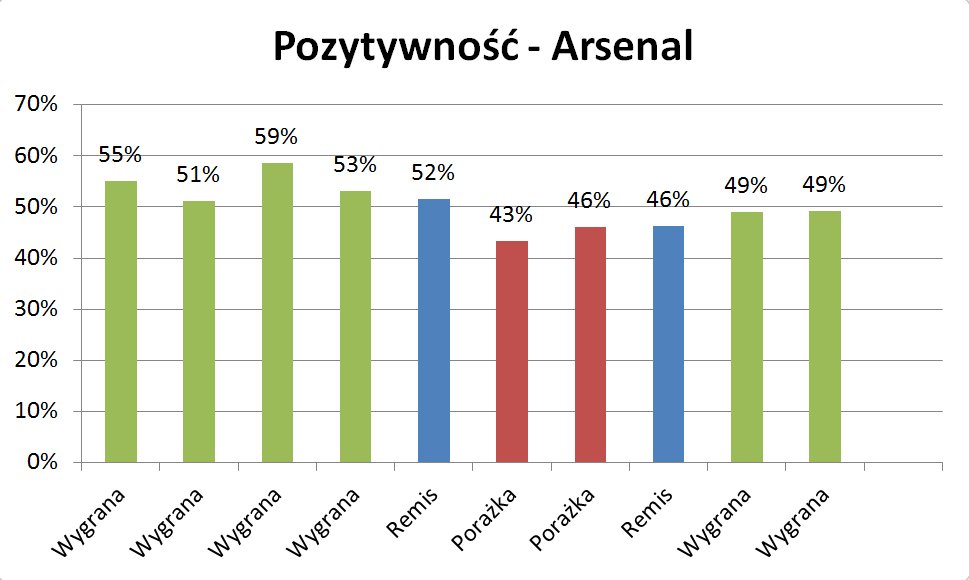
\includegraphics[width=120mm]{img/pozytywnosc-arsenal.png}
\caption{Wyniki spotkań Arsenalu a sentyment wpisów}
\label{image:pozytywnosc-arsenal}
\end{figure}


\begin{figure}[ht!]
\centering
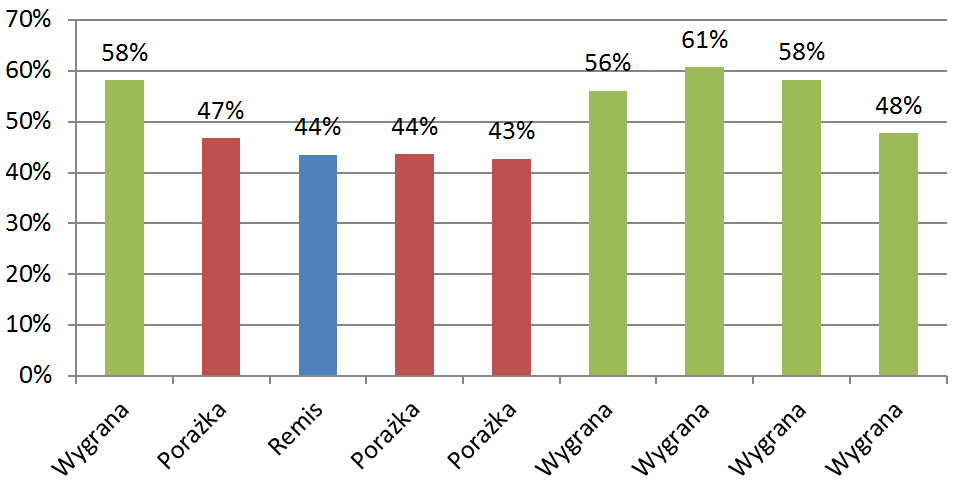
\includegraphics[width=120mm]{img/pozytywnosc-munited.png}
\caption{Wyniki spotkań Manchesteru United a sentyment wpisów}
\label{image:pozytywnosc-munited}
\end{figure}

\clearpage
\subsubsection{Obserwacje i wnioski}
Posiadając informację na temat końcowego wyniku danego meczu łatwo można 
zauważyć, iż wartość sentymentu jest adekwatna do uzyskanego rezultatu danej 
drużyny. Gdy Arsenal odnosi zwycięstwo wówczas wpisy mają częściej wydźwięk
pozytywny przekraczając w większości przypadków wartość 50\%. Gdy jednak 
drużyna przegrywa nacechowanie emocjonalne wpisów wyraźnie spada poniżej 46\%.
Również mecz zakończony remisem powoduje raczej wpisy niezadowolenia.
 
Tę samą prawidłowość można zauważyć analizując wyniki badań dla meczów
Manchesteru United. Gdy drużyna wygrywa, wówczas zadowolenia we wpisach sięga
nawet 61\%, a gdy ponosi porażkę -- wynik sentymentu spada do czterdziestu kilku
procent.

Po analizie tych badań nasuwają się oczywiste wnioski. Sposób reagowania
internautów na wyniki ich drużyn jest dokładnie taki sam jak rezultat przez nie
osiągany. Gdy drużyna wygrywa, okazuje się lepsza, to tak samo jak w życiu, jej
kibice wykazują radość, szczęście, zadowolenie i inne pozytywne emocje.
Natomiast gdy klub przegrywa mecz, wówczas wśród tweetów dużo łatwiej o wpisy o
nacechowaniu negatywnym. Widać więc, że reakcje użytkowników Twittera są
dokładnie takie same jak zwykłych kibiców -- odzwierciedlają ich aktualny stan
ducha po meczu ulubionej drużyny. Nie ma tutaj żadnej różnicy między światem
realnym a wirtualnym.

\bigskip
Szersze zastosowanie analizy sentymentu zostało wykorzystane w kolejnych
badaniach zaprezentowanych poniżej.






















%%%%%%%%%%%%%%%%%%%%%%%%%%%%%%%%%%%%%%%%%%%%%%%%%%%%%%%%%%%%%% ANALIZA SPOŁECZNA
\clearpage
\section{Analiza sieci społecznych}
\label{section:analizaspoleczna}
Do analizy sieci społecznych zostały użyte dane użytkowników pobrane 
równocześnie ze ściąganiem wpisów. Relacje między użytkownikami zostały
zbudowane na podstawie informacji zawartych w tweetach. Są to więc
dwa rodzaje relacji -- odpowiedzi i retweety. Z ich pomocą przeprowadzone
zostały badania nad siecią społeczną, którą tworzą użytkownicy Twittera. 






\subsection{Liczba i rodzaje komunikacji między zwolennikami i przeciwnikami klubów}
% retweety pozytywne zwolennicy, replies negatywne, przeciwnicy, itd

Jednym z eksperymentów przeprowadzonych w analizie sieci społecznych było
sprawdzenie rodzaju komunikacji pomiędzy użytkownikami. Aby jednak wzbogacić
ten eksperyment użyty został zbadany wcześniej sentyment. Przy jego pomocy
oznaczono każdego użytkownika jako przeciwnika lub zwolennika danego klubu.

\subsubsection{Wykrywanie zwolenników i przeciwników klubu}
Proces oznaczania użytkowników jako sympatyków i przeciwników drużyny przebiegał
w następujący sposób:
\begin{itemize}
  \item dla każdego użytkownika zliczono jego wpisy w meczach każdej z czterech 
  drużyn,
  \item jeśli w meczach drużyny A dla danego użytkownika przeważała liczba 
  wpisów pozytywnych, wówczas oznaczano takiego kibica jako zwolennika drużyny A,
  \item jeśli natomiast przeważała liczba wpisów negatywnych, wówczas taki kibic
  traktowany był jako przeciwnik danej drużyny.  
\end{itemize} 


\clearpage
\subsubsection{Charakterystyka komunikacji poprzez odpowiedzi (\textit{replies})}
Zbadana został sposób w jaki komunikują się użytkownicy Twittera korzystając
z funkcji \textit{odpowiedz}, polegającej na możliwości komentowania wpisów
innych użytkowników. Tak jak było to wcześniej zaznaczone w tym serwisie
społecznościowym użytkownicy dowoli mogą komentować wpisy osób, których
nie mają na swoich listach znajomych.

Poprzez podzielenie użytkowników na grupy zwolenników i przeciwników -- na
przykładzie wpisów dotyczących Manchesteru United -- można zauważyć ciekawe
obserwacje. Wykres przedstawiający wyniki badań przedstawia rysunek 
\ref{image:replies-munited}.


\begin{figure}[ht!]
\centering
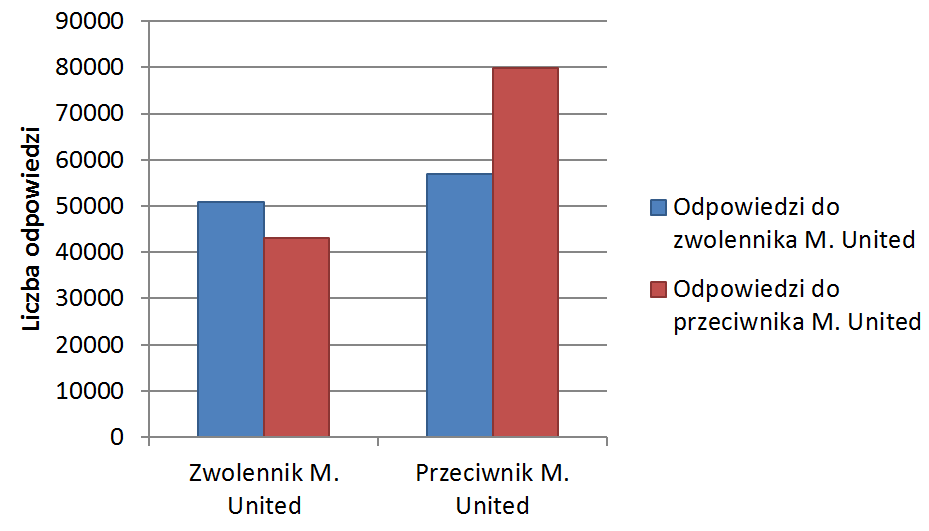
\includegraphics[width=120mm]{img/replies-munited.png}
\caption{Charakterystyka odpowiedzi wśród wpisów dotyczących Manchesteru United}
\label{image:replies-munited}
\end{figure}

\subsubsection{Obserwacje i wnioski}
Wykres przedstawia liczbę odpowiedzi zwolenników i przeciwników Manchesteru 
United na wpisy zwolenników i przeciwników tego klubu. Na jego podstawie można
zauważyć, że na wpisy zwolenników częściej odpowiadają zwolennicy. 
Oznacza to, że ta grupa użytkowników trzyma się blisko siebie i osoby, które
są sympatykami Manchesteru również obserwują i komunikują się z innymi 
sympatykami tego klubu produkując większą liczbę wpisów.
Podobna zależność ma miejsce wśród przeciwników Manchesteru United.
Wpis przeciwnika tego klubu bardziej angażuje do dyskusji również innych
przeciwników. Prawdopodobnie osoby biorące udział w tej dyskusji wspólnie
narzekają na grę tego zespołu, wzajemnie nakręcając się do ożywionych dyskusji.

Na podstawie powyższego wykresu widać więc, że użytkownicy Twittera lubią 
tworzyć grupy o podobnych zainteresowaniach czy sympatiach. Dany użytkownik
częściej będzie komunikował się z osobami, które myślą podobnie jak on,
umacniając w ten sposób swoje przekonanie o własnych przemyśleniach na dany temat.
Gdy ktoś jest zwolennikiem danego klubu częściej dyskutuje z podobnymi sobie
internautami. Tak samo przeciwnicy łatwiej znajdują nić porozumienia między sobą
mając takie samo zdanie dotyczące określonego wydarzenia. Internauci lepiej
odnajdują się wśród osób podzielających ich opinie.  









\subsubsection{Charakterystyka komunikacji poprzez retweety}
Podobnie jak powyższe badanie został przeprowadzony eksperyment na temat 
charakterystyki komunikacji między użytkownikami korzystający z opcji 
\textit{retweet}. Polega ona na podaniu dalej wpisu, który uważamy za ciekawy.
Wyniki, które w ten sposób uzyskano różnią się od poprzednich i zaprezentowane
są na rysunku \ref{image:retweety-munited}.

\begin{figure}[ht!]
\centering
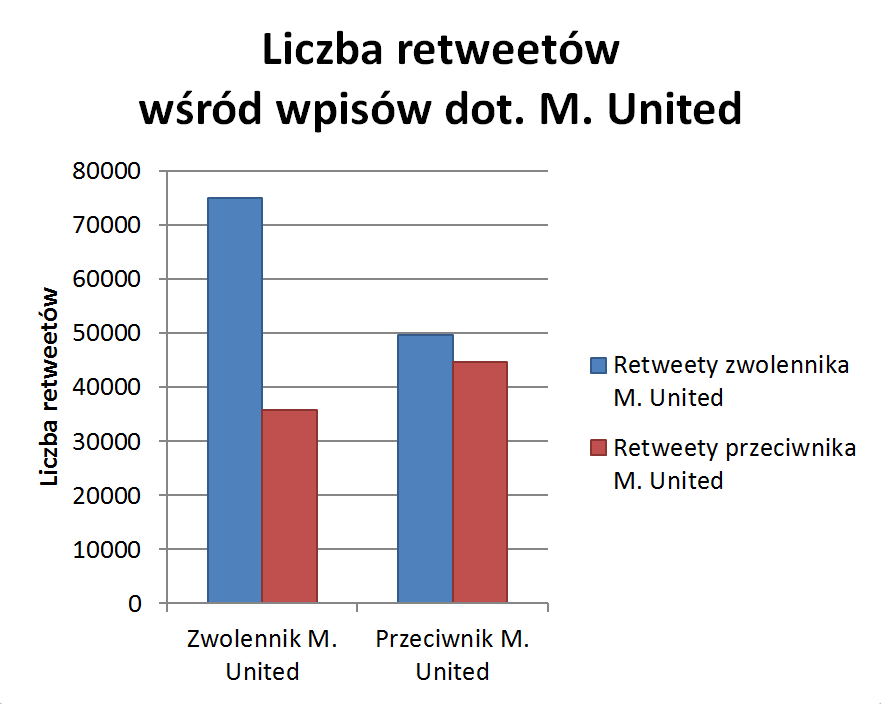
\includegraphics[width=120mm]{img/retweety-munited.png}
\caption{Charakterystyka retweetów wśród wpisów dotyczących Manchesteru United}
\label{image:retweety-munited}
\end{figure}



\subsubsection{Obserwacje i wnioski}
%Zwolennicy najczęściej retweetują wpisy zwolenników \ref{image:retweety-munited}
Tym razem widać zupełnie inne ułożenie słupków na wykresie.
Na pierwszy plan wyraźnie wysuwa się słupek pierwszy z lewej, który oznacza
liczbę wpisów zwolenników podanych dalej przez innych zwolenników. Widać więc,
że sympatycy Manchesteru United bardzo chętnie przekazują dalej wpisy 
pozostałych sympatyków. Mogą to być na przykład wpisy o strzelonym golu,
czy jakieś pozytywne opinie na temat danej drużyny. Najrzadziej z całej
czwórki zaprezentowanych relacji dochodzi do sytuacji, gdy przeciwnik
Manchseteru podaje dalej wpis zwolennika. Jeśli chodzi o retweetowanie
tweetów przeciwników Manchesteru United, to dochodzi do tego mniej więcej po
równo między przeciwnikami i zwolennikami.

Po analizie dwóch powyższych eksperymentów nasuwają się następujące wnioski.
Użytkownicy lubią gromadzić się w grupy o podobnych zainteresowaniach,
wspólnie komentując wydarzenia w podobny sposób. Zwolennicy i przeciwnicy
danego klubu zachowują się w charakterystyczny sposób. Ci pierwsi bardzo często
retweetują wpisy innych zwolenników, a ci drudzy częściej dyskutują ze sobą.

































\clearpage
\subsection{Sentyment odpowiedzi między zwolennikami i przeciwnikami drużyny}

\subsubsection{Gdy odpowiada zwolennik Arsenalu}

Zwolennicy bardzo często odpowiadają innym zwolennikom na wpisy pozytywne,
również wpisami pozytywnymi \ref{image:reply-sentiment-zwolennik-zwolennik}.
\begin{figure}[ht!]
\centering
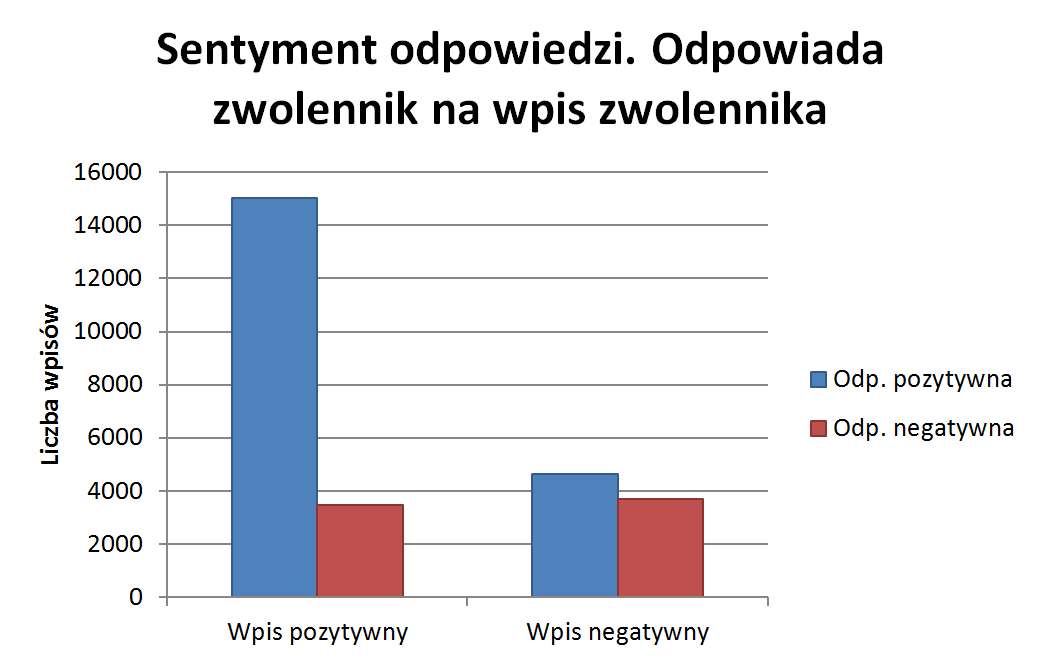
\includegraphics[width=120mm]{img/reply-sentiment-zwolennik-zwolennik.png}
\caption{Sentyment odpowiedzi}
\label{image:reply-sentiment-zwolennik-zwolennik}
\end{figure}

Zwolennicy nawet na wpisy negatywne starają się odpowiadać pozytywnie
 \ref{image:reply-sentiment-zwolennik-przeciwnik}.
 
\begin{figure}[ht!]
\centering
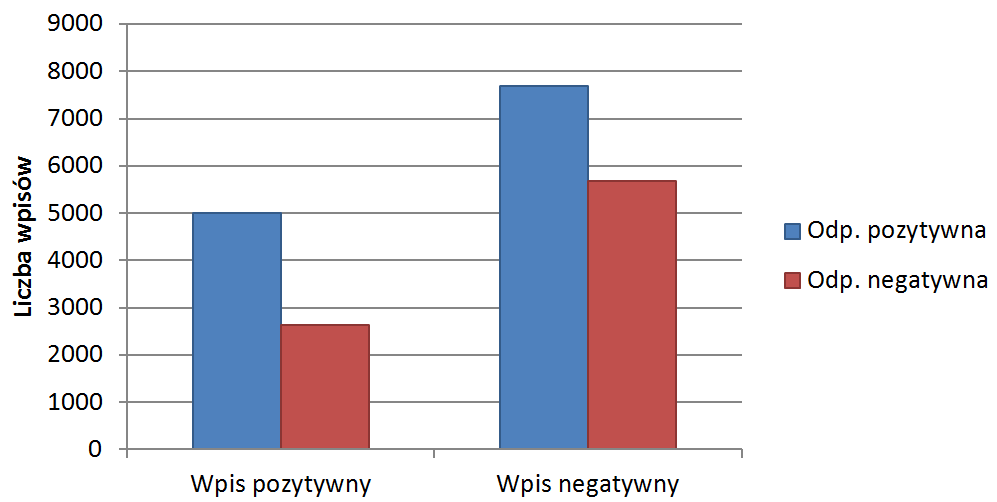
\includegraphics[width=120mm]{img/reply-sentiment-zwolennik-przeciwnik.png}
\caption{Sentyment odpowiedzi}
\label{image:reply-sentiment-zwolennik-przeciwnik}
\end{figure}


\clearpage
\subsubsection{Gdy odpowiada przeciwnik Arsenalu}

Przeciwnicy odpowiadają negatywnie zwolennikom zarówno na wpisy pozytywne jak 
i negatywne \ref{image:reply-sentiment-przeciwnik-zwolennik}.

\begin{figure}[ht!] \centering
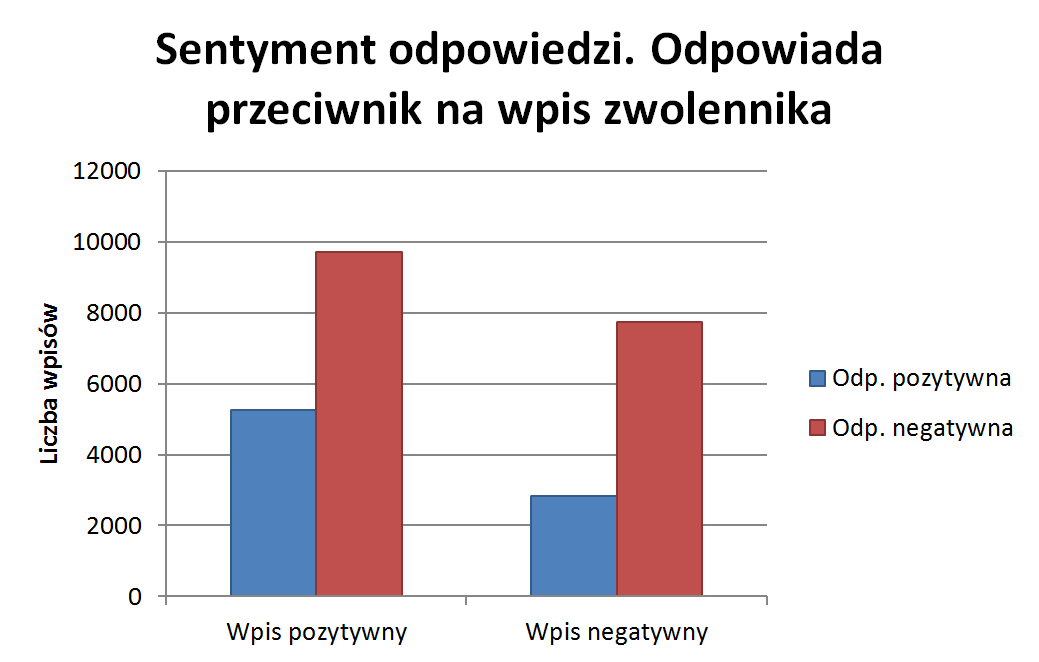
\includegraphics[width=120mm]{img/reply-sentiment-przeciwnik-zwolennik.png}
\caption{Sentyment odpowiedzi}
\label{image:reply-sentiment-przeciwnik-zwolennik}
\end{figure}


Przeciwnicy klubu najchętniej odpowiadają innym przeciwnikom na wpisy negatywne
wpisami negatywnymi \ref{image:reply-sentiment-przeciwnik-przeciwnik}.

\begin{figure}[ht!] \centering
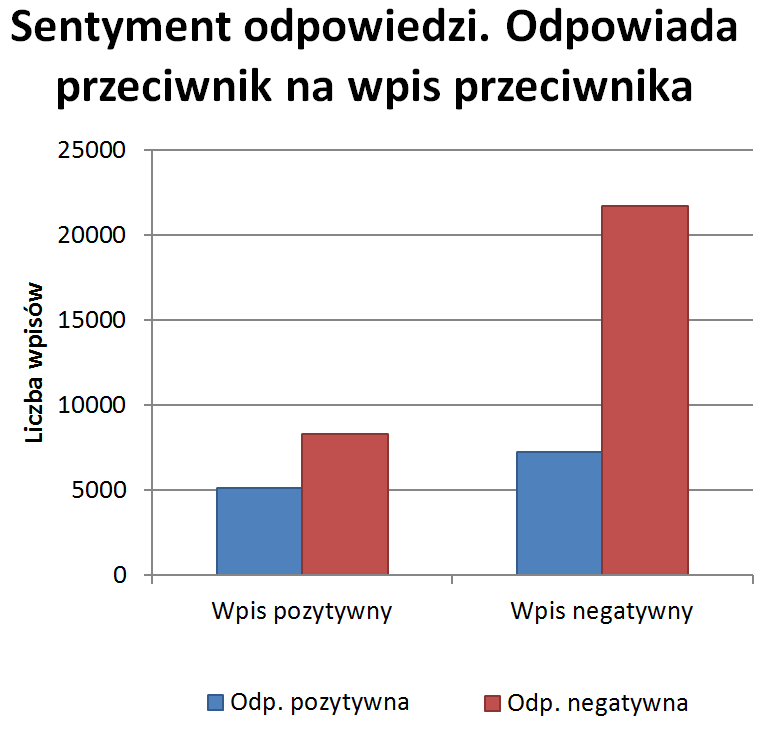
\includegraphics[width=120mm]{img/reply-sentiment-przeciwnik-przeciwnik.png}
\caption{Sentyment odpowiedzi}
\label{image:reply-sentiment-przeciwnik-przeciwnik}
\end{figure}










%%%%%%%%%%%%%%%%%%%%
Podobieństwo w meczach Arsenalu \ref{image:grupy-arsenal}
 
\begin{figure}[ht!]
\centering
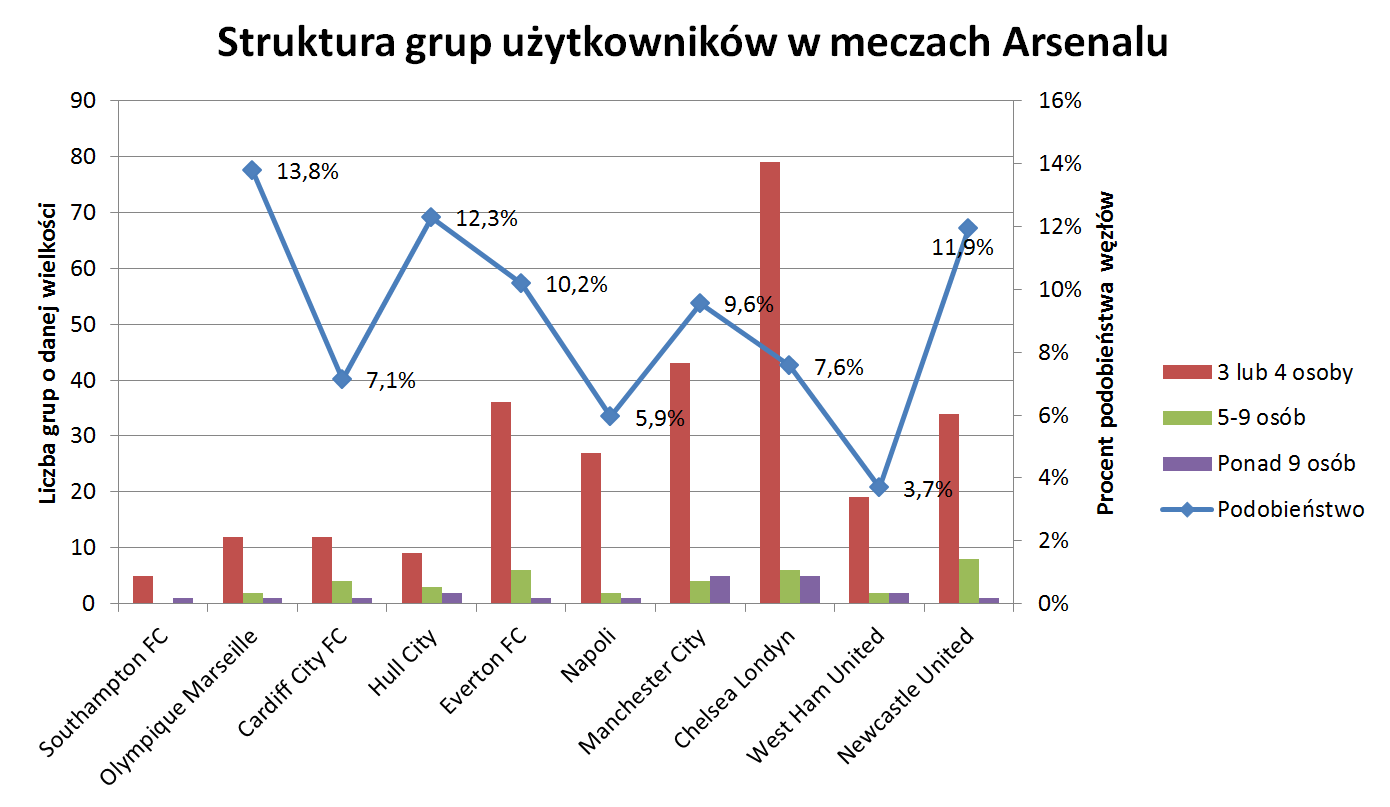
\includegraphics[width=120mm]{img/grupy-arsenal.png}
\caption{Struktura grup użytkowników w meczach Arsenalu}
\label{image:grupy-arsenal}
\end{figure}

Podobieństwo w meczach Manchesteru United \ref{image:grupy-munited}

\begin{figure}[ht!]
\centering
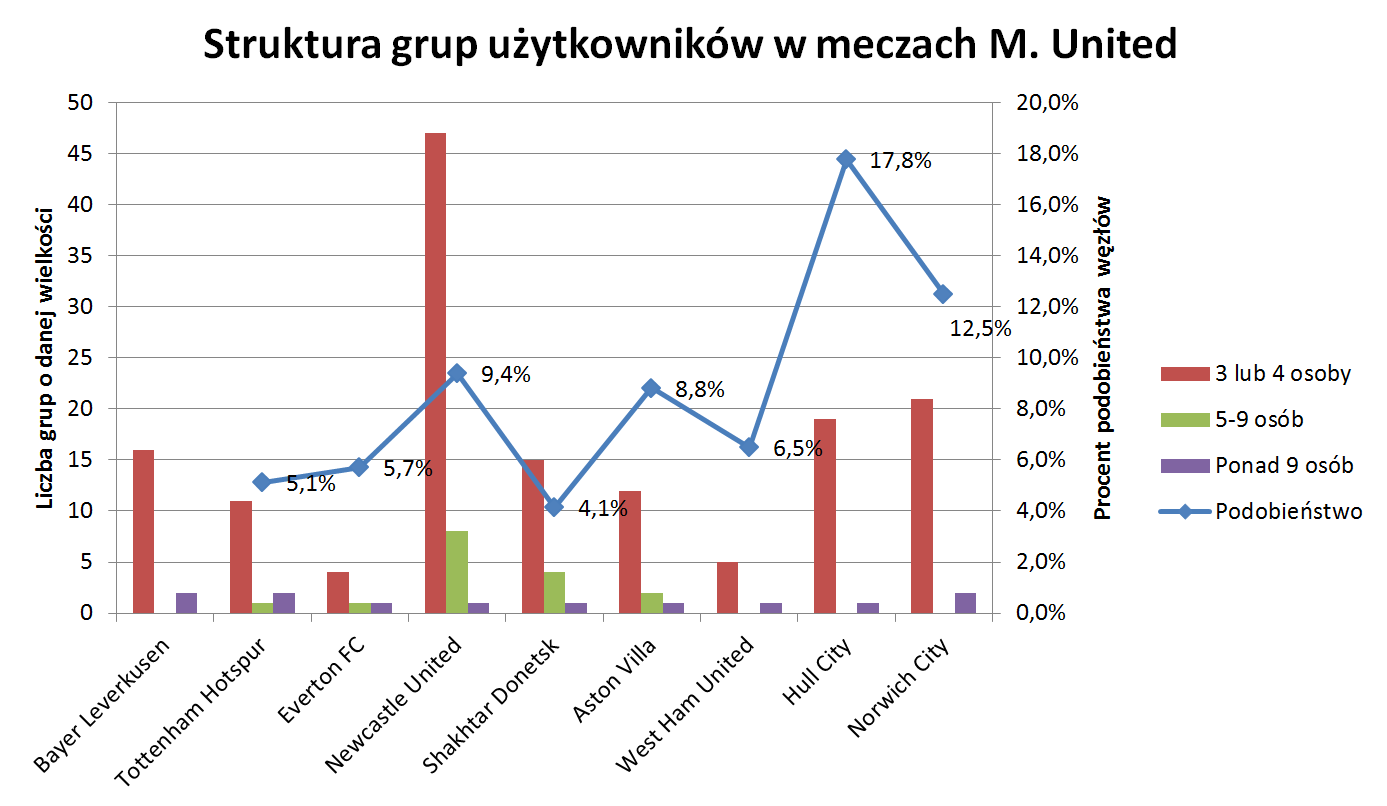
\includegraphics[width=120mm]{img/grupy-munited.png}
\caption{Struktura grup użytkowników w meczach Manchesteru United}
\label{image:grupy-munited}
\end{figure}

% Podobieństwo węzłów między meczami 
% Podobieństwo grafów między meczami 
% Między mało popularnymi spotkaniami wysoki stopień podobieństwa
% +Sentyment a wielkość grupy











%%%%%%%%%%%%%%%%%%%%%%%%%%%%%%%%%%%%%%%%%%%%%%%%%%%%%%%%%% ANALIZA GEOGRAFICZNA
\clearpage
\section{Analiza geograficzna}
\label{section:analizageograficzna}
%Odległość użytkowników komunikujących się ze sobą od siebie

Im kibice są fizycznie bliżej siebie, tym częściej się ze sobą komunikują, 
co przedstawia poniższy wykres \ref{image:relacje-a-odleglosc}.
Wartości odległości w kolejnych kolumnach rosną wykładniczo,
a liczba użytkowników, między którymi doszło do wymiany wiadomości
pozostaje na takim samym rzędzie wielkości. Między użytkownikami oddalonymi
od siebie o maksymalnie 10 km doszło do tylu samo wymian wiadomości,
jak między użytkownikami oddalonymi od 10 do 100 km, czy między użytkownikami
oddalonymi od 100 do 1000 km od siebie.

\begin{figure}[ht!]
\centering
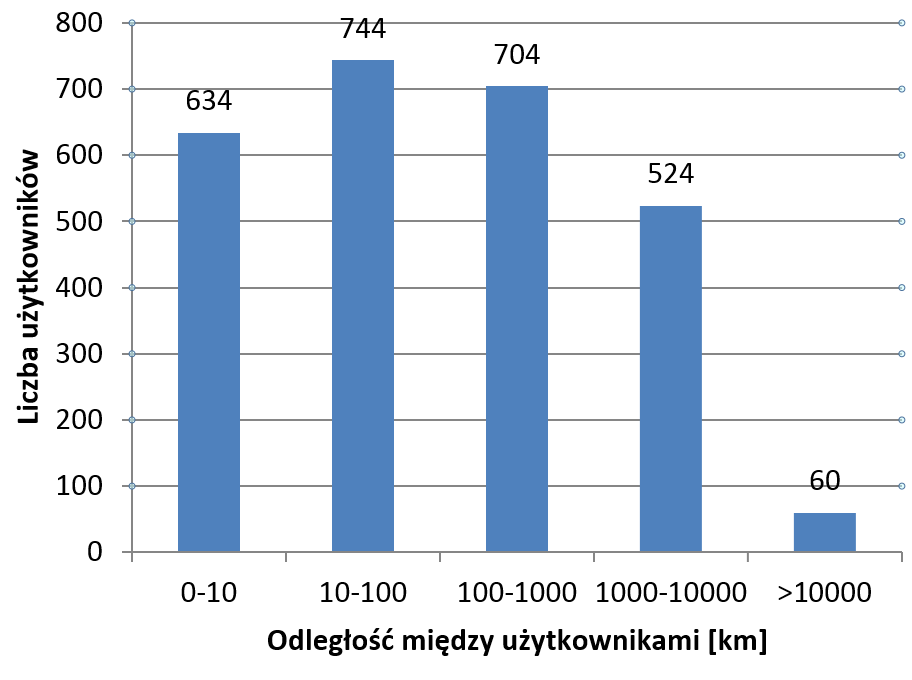
\includegraphics[width=120mm]{img/relacje-a-odleglosc.png}
\caption{Relacje między użytkownikami a odległość fizyczna między nimi}
\label{image:relacje-a-odleglosc}
\end{figure}

%Odległość od stadionu zwolenników, przeciwników 
%Odległość od stadionu a sentyment
%Miejscowości a sentyment 
%Kraje, a sentyment




